
%% bare_conf_compsoc.tex
%% V1.4b
%% 2015/08/26
%% by Michael Shell
%% See:
%% http://www.michaelshell.org/
%% for current contact information.
%%
%% This is a skeleton file demonstrating the use of IEEEtran.cls
%% (requires IEEEtran.cls version 1.8b or later) with an IEEE Computer
%% Society conference paper.
%%
%% Support sites:
%% http://www.michaelshell.org/tex/ieeetran/
%% http://www.ctan.org/pkg/ieeetran
%% and
%% http://www.ieee.org/

%%*************************************************************************
%% Legal Notice:
%% This code is offered as-is without any warranty either expressed or
%% implied; without even the implied warranty of MERCHANTABILITY or
%% FITNESS FOR A PARTICULAR PURPOSE!
%% User assumes all risk.
%% In no event shall the IEEE or any contributor to this code be liable for
%% any damages or losses, including, but not limited to, incidental,
%% consequential, or any other damages, resulting from the use or misuse
%% of any information contained here.
%%
%% All comments are the opinions of their respective authors and are not
%% necessarily endorsed by the IEEE.
%%
%% This work is distributed under the LaTeX Project Public License (LPPL)
%% ( http://www.latex-project.org/ ) version 1.3, and may be freely used,
%% distributed and modified. A copy of the LPPL, version 1.3, is included
%% in the base LaTeX documentation of all distributions of LaTeX released
%% 2003/12/01 or later.
%% Retain all contribution notices and credits.
%% ** Modified files should be clearly indicated as such, including  **
%% ** renaming them and changing author support contact information. **
%%*************************************************************************


% *** Authors should verify (and, if needed, correct) their LaTeX system  ***
% *** with the testflow diagnostic prior to trusting their LaTeX platform ***
% *** with production work. The IEEE's font choices and paper sizes can   ***
% *** trigger bugs that do not appear when using other class files.       ***                          ***
% The testflow support page is at:
% http://www.michaelshell.org/tex/testflow/



\documentclass[conference,compsoc]{IEEEtran}
% Some/most Computer Society conferences require the compsoc mode option,
% but others may want the standard conference format.
%
% If IEEEtran.cls has not been installed into the LaTeX system files,
% manually specify the path to it like:
% \documentclass[conference,compsoc]{../sty/IEEEtran}





% Some very useful LaTeX packages include:
% (uncomment the ones you want to load)


% *** MISC UTILITY PACKAGES ***
%
%\usepackage{ifpdf}
% Heiko Oberdiek's ifpdf.sty is very useful if you need conditional
% compilation based on whether the output is pdf or dvi.
% usage:
% \ifpdf
%   % pdf code
% \else
%   % dvi code
% \fi
% The latest version of ifpdf.sty can be obtained from:
% http://www.ctan.org/pkg/ifpdf
% Also, note that IEEEtran.cls V1.7 and later provides a builtin
% \ifCLASSINFOpdf conditional that works the same way.
% When switching from latex to pdflatex and vice-versa, the compiler may
% have to be run twice to clear warning/error messages.






% *** CITATION PACKAGES ***
%
\ifCLASSOPTIONcompsoc
  % IEEE Computer Society needs nocompress option
  % requires cite.sty v4.0 or later (November 2003)
  \usepackage[nocompress]{cite}
\else
  % normal IEEE
  \usepackage{cite}
\fi
% cite.sty was written by Donald Arseneau
% V1.6 and later of IEEEtran pre-defines the format of the cite.sty package
% \cite{} output to follow that of the IEEE. Loading the cite package will
% result in citation numbers being automatically sorted and properly
% "compressed/ranged". e.g., [1], [9], [2], [7], [5], [6] without using
% cite.sty will become [1], [2], [5]--[7], [9] using cite.sty. cite.sty's
% \cite will automatically add leading space, if needed. Use cite.sty's
% noadjust option (cite.sty V3.8 and later) if you want to turn this off
% such as if a citation ever needs to be enclosed in parenthesis.
% cite.sty is already installed on most LaTeX systems. Be sure and use
% version 5.0 (2009-03-20) and later if using hyperref.sty.
% The latest version can be obtained at:
% http://www.ctan.org/pkg/cite
% The documentation is contained in the cite.sty file itself.
%
% Note that some packages require special options to format as the Computer
% Society requires. In particular, Computer Society  papers do not use
% compressed citation ranges as is done in typical IEEE papers
% (e.g., [1]-[4]). Instead, they list every citation separately in order
% (e.g., [1], [2], [3], [4]). To get the latter we need to load the cite
% package with the nocompress option which is supported by cite.sty v4.0
% and later.





% *** GRAPHICS RELATED PACKAGES ***
%
\ifCLASSINFOpdf
   \usepackage[pdftex]{graphicx}
  % declare the path(s) where your graphic files are
  % \graphicspath{{../pdf/}{../jpeg/}}
  % and their extensions so you won't have to specify these with
  % every instance of \includegraphics
  % \DeclareGraphicsExtensions{.pdf,.jpeg,.png}
\else
  % or other class option (dvipsone, dvipdf, if not using dvips). graphicx
  % will default to the driver specified in the system graphics.cfg if no
  % driver is specified.
  % \usepackage[dvips]{graphicx}
  % declare the path(s) where your graphic files are
  % \graphicspath{{../eps/}}
  % and their extensions so you won't have to specify these with
  % every instance of \includegraphics
  % \DeclareGraphicsExtensions{.eps}
\fi
% graphicx was written by David Carlisle and Sebastian Rahtz. It is
% required if you want graphics, photos, etc. graphicx.sty is already
% installed on most LaTeX systems. The latest version and documentation
% can be obtained at:
% http://www.ctan.org/pkg/graphicx
% Another good source of documentation is "Using Imported Graphics in
% LaTeX2e" by Keith Reckdahl which can be found at:
% http://www.ctan.org/pkg/epslatex
%
% latex, and pdflatex in dvi mode, support graphics in encapsulated
% postscript (.eps) format. pdflatex in pdf mode supports graphics
% in .pdf, .jpeg, .png and .mps (metapost) formats. Users should ensure
% that all non-photo figures use a vector format (.eps, .pdf, .mps) and
% not a bitmapped formats (.jpeg, .png). The IEEE frowns on bitmapped formats
% which can result in "jaggedy"/blurry rendering of lines and letters as
% well as large increases in file sizes.
%
% You can find documentation about the pdfTeX application at:
% http://www.tug.org/applications/pdftex
\usepackage[utf8]{inputenc}
%\usepackage[english]{babel}
\usepackage[english]{babel}


\usepackage{amsthm}

\renewcommand{\qedsymbol}{$\blacksquare$}

\newtheorem{thm}{Theorem}%[section]
\newtheorem{lem}[thm]{Lemma}
\newtheorem{prop}[thm]{Proposition}
\newtheorem{cor}{Corollary}
\newtheorem{conj}{Conjecture}[section]
\theoremstyle{definition}
\newtheorem{defn}{Definition}[section]
\newtheorem{exmp}{Example}[section]
\newtheorem{rem}{Remark}





\usepackage{algorithm}
\usepackage[noend]{algpseudocode}

\makeatletter
\def\BState{\State\hskip-\ALG@thistlm}
\makeatother

% *** MATH PACKAGES ***
%
 \usepackage{amssymb}
\usepackage{amsmath}
% A popular package from the American Mathematical Society that provides
% many useful and powerful commands for dealing with mathematics.
%
% Note that the amsmath package sets \interdisplaylinepenalty to 10000
% thus preventing page breaks from occurring within multiline equations. Use:
%\interdisplaylinepenalty=2500
% after loading amsmath to restore such page breaks as IEEEtran.cls normally
% does. amsmath.sty is already installed on most LaTeX systems. The latest
% version and documentation can be obtained at:
% http://www.ctan.org/pkg/amsmath





% *** SPECIALIZED LIST PACKAGES ***
%
%\usepackage{algorithmic}
% algorithmic.sty was written by Peter Williams and Rogerio Brito.
% This package provides an algorithmic environment fo describing algorithms.
% You can use the algorithmic environment in-text or within a figure
% environment to provide for a floating algorithm. Do NOT use the algorithm
% floating environment provided by algorithm.sty (by the same authors) or
% algorithm2e.sty (by Christophe Fiorio) as the IEEE does not use dedicated
% algorithm float types and packages that provide these will not provide
% correct IEEE style captions. The latest version and documentation of
% algorithmic.sty can be obtained at:
% http://www.ctan.org/pkg/algorithms
% Also of interest may be the (relatively newer and more customizable)
% algorithmicx.sty package by Szasz Janos:
% http://www.ctan.org/pkg/algorithmicx




% *** ALIGNMENT PACKAGES ***
%
%\usepackage{array}
% Frank Mittelbach's and David Carlisle's array.sty patches and improves
% the standard LaTeX2e array and tabular environments to provide better
% appearance and additional user controls. As the default LaTeX2e table
% generation code is lacking to the point of almost being broken with
% respect to the quality of the end results, all users are strongly
% advised to use an enhanced (at the very least that provided by array.sty)
% set of table tools. array.sty is already installed on most systems. The
% latest version and documentation can be obtained at:
% http://www.ctan.org/pkg/array


% IEEEtran contains the IEEEeqnarray family of commands that can be used to
% generate multiline equations as well as matrices, tables, etc., of high
% quality.



% correct bad hyphenation here
\hyphenation{op-tical net-works semi-conduc-tor}


\begin{document}
%

\algnewcommand\algorithmicswitch{\textbf{switch}}
\algnewcommand\algorithmiccase{\textbf{case}}
\algnewcommand\algorithmicassert{\texttt{assert}}
\algnewcommand\Assert[1]{\State \algorithmicassert(#1)}%
% New "environments"
\algdef{SE}[SWITCH]{Switch}{EndSwitch}[1]{\algorithmicswitch\ #1\ \algorithmicdo}{\algorithmicend\ \algorithmicswitch}%
\algdef{SE}[CASE]{Case}{EndCase}[1]{\algorithmiccase\ #1}{\algorithmicend\ \algorithmiccase}%
\algtext*{EndSwitch}%
\algtext*{EndCase}%

% paper title
% Titles are generally capitalized except for words such as a, an, and, as,
% at, but, by, for, in, nor, of, on, or, the, to and up, which are usually
% not capitalized unless they are the first or last word of the title.
% Linebreaks \\ can be used within to get better formatting as desired.
% Do not put math or special symbols in the title.
%\title{An Optimized-Location and Optimized-Power Scheme for Fog-based IoT Networks}
%\title{Mobile Edge Computing in Fog-based Internet-of-Things (IoT) Networks}
\title{Fog-assisted Communication in Mobile Edge Computing-based Internet-of-Things (IoT) Networks}
% author names and affiliations
% use a multiple column layout for up to three different
% affiliations
\author{\IEEEauthorblockN{zzz ttt}
\IEEEauthorblockA{%Computer Science Programme\\
Trinity College Dublin\\
Ireland\\
Email: yy@tcd.ie}
\and
\IEEEauthorblockN{ppp kkk, and rrr yyy}
\IEEEauthorblockA{
Trinity College Dublin\\
Ireland\\
Email: xx@tcd.ie}}


% make the title area
\maketitle

% As a general rule, do not put math, special symbols or citations
% in the abstract
\begin{abstract}

Mobile edge computing (MEC) offers an information and communication technology environment with cloud computing capabilities within the radio access network (RAN). With increasing demand on real-time services, high-bandwidth, ultra-low latency, and minimal energy consumption from a massive number of devices, the fog-based Internet-of-things and MEC framework both have the potential to offer real-time, context-aware processing, and personalized services by leveraging proximity to end-users. However, mobility brings about several bottlenecks that hamper communication reliability within a network. This paper examines the uplink communication performance of an IoT end-device that leverages on a fog device, such as a 5G-enabled mobile device, to offload tasks to a remote MEC server situated at a macro base station. Putting into consideration the channel variations due to mobility of the fog device, we present a closed-form analytical expression for the achievable data rate. We then apply the stochastic gradient ascent optimization algorithm to the formulated problem in order to achieve convergence. Simulation results show an improved learning in the proposed algorithm.

\end{abstract}

\begin{IEEEkeywords}
Mobile edge computing, fog, Internet-of-things, stochastic gradient ascent, optimization.
\end{IEEEkeywords}

\IEEEpeerreviewmaketitle


\section{Introduction}
Mobile edge computing (MEC) has brought about immense potentials that could be derived from the 5G technology. Driven by diverse use cases such as the Internet of Things (IoT), public safety, explosive data usage, extreme video and gaming applications, and context-aware services, 5G brings about extreme requirements to the network. These requirements range from massive broadband to critical machine communication. As such, MEC will be a key building block in the evolution of mobile broadband and a fundamental technology and architectural concept. MEC entails hosting third-party authorized applications in the operator's network and allows for a synergy, where network providers and content providers can collaborate to provide an improved user experience. The MEC gives room for content developers to provide context-aware services by leveraging the real-time radio access network (RAN) information from MEC.

The emergence of MEC seems to have brought a lasting solution to imminent challenges such as high latency, slower application speed, and link failures, that often characterize the mobile cloud computing paradigm, however, distribution and allocation of computing resources, decisions on where and how to offload in cases of mobility and channel variations, remain a challenge in MEC~\cite{Yu2016}.
Designing a resilient network involves more than the addition of redundant links, it entails minimizing the communication outage by countervailing the impact of the wireless channel. In energy and resource-constrained environment such as IoT, it is often necessary for the IoT end-devices to offload some computation-intensive task unto a remote device or server. This device may not necessarily be situated in the far-away cloud, rather, it could be at the edge of the network. Several researchers~\cite{Lin16},~\cite{Chiang16} have highlighted the need to integrate the fog/edge computing paradigm with the IoT, in view of actualizing the IoT vision. The fog/edge computing based IoT (FECIoT) has the potential to meet the growing demands on real-time processing and data analytics.

The term ``FECIoT'' was first coined by Lin \textit{et al.} in~\cite{Lin16} with a motive to emphasize the immense potential that could be derived by integrating the fog/edge computing paradigm with the IoT architecture. The FECIoT framework consists of IoT end-devices, highly distributed and hierarchically-placed fog/edge devices, and the centralized cloud infrastructure~\cite{Chiang16}. Recently, the European Telecommunications Standards Institute (ETSI) MEC Industry Specification Group (ISG), was set up to find ways of standardizing the MEC to become an integral part of 5G systems driven by IoT. The ETSI MEC ISG was assigned the task of producing a set of specifications to allow third-party authorized applications to be hosted in a multi-vendor environment~\cite{Sabella16}. Questions may arise as to what roles MEC will play in the new FECIoT architectural framework. The MEC can readily be deployed in a distributed manner, leveraging on existing cellular infrastructures. Likewise, the FECIoT framework supports service provisioning at the edge of the network, with better prospects for small-to-medium-sized enterprises (SMEs).



In this paper, we consider an uplink communication scenario between an IoT end-device and the MEC server via a 5G-enabled fog device, usually a smartphone. We formulate an optimization problem that maximizes the achievable data rate, and then applied a stochastic gradient ascent optimization algorithm to improve the communication performance of the proposed scenario.

\section{System Model}
In this paper, we consider an uplink communication scenario as shown in Figure~\ref{MECmodel}, where an IoT end-device offloads data or service request to the MEC server via a 5G-enabled fog device, usually a smartphone.



\begin{figure}[!t]
\centering
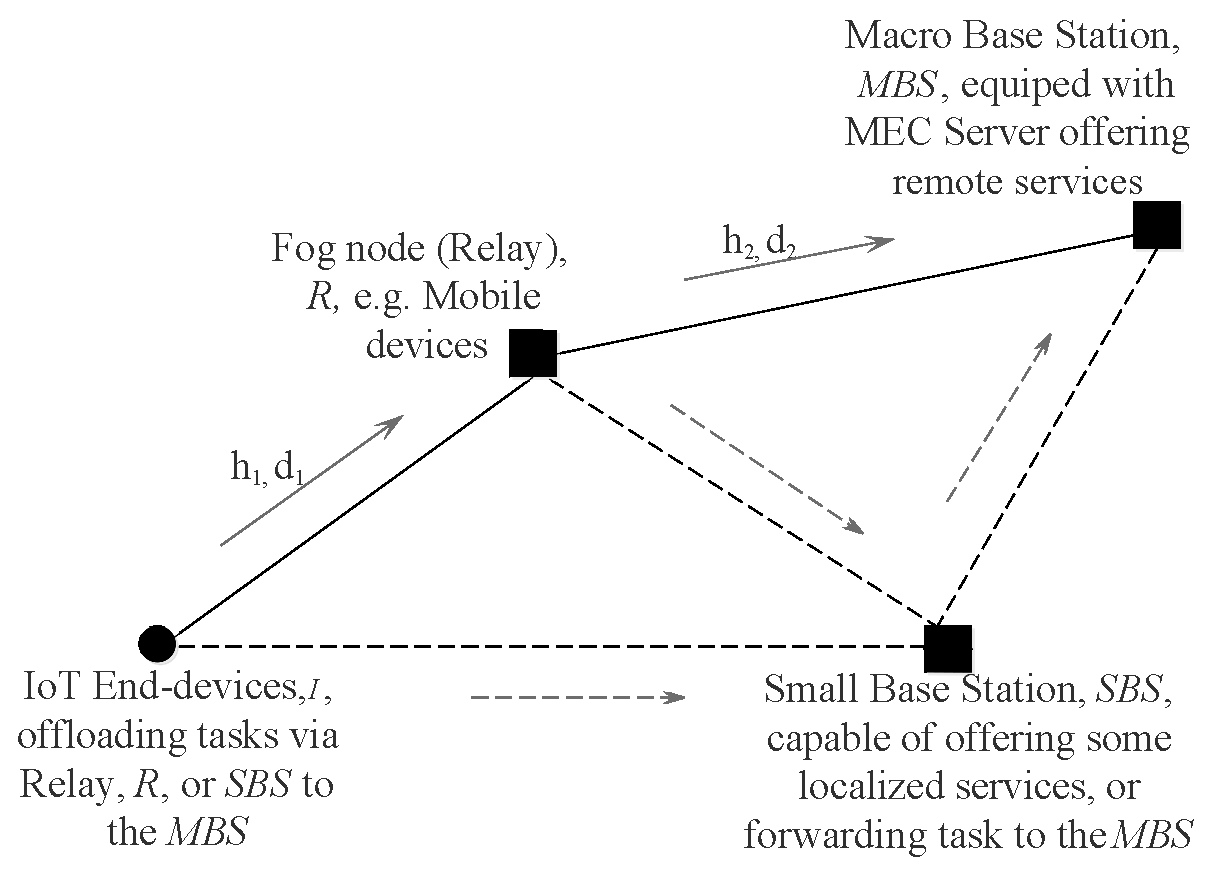
\includegraphics[width=3.5in]{MECmodel.eps}
 %where an .eps filename suffix will be assumed under latex,
% and a .pdf suffix will be assumed for pdflatex; or what has been declared
% via \DeclareGraphicsExtensions.
\caption{System model.}
\label{MECmodel}
\end{figure}


\section{Optimization}





\section{Results}
Table \ref{table:parameters} shows the simulation parameters used in our analysis.
\begin{table}
\small
\centering
\caption{Simulation Parameters}
\label{table:parameters}
\begin{tabular}{ll}
  \hline
 \textit{Parameters} & \textit{Value} \\
  \hline \hline
   Iterations & 1000\\
   Number of simulations & 400\\
   Maximum transmit power~$P_{max}$  & 20 \emph{dBm}\\
   Noise power~$N_0$ & $-99$ \emph{dBm}\\
   Path-loss exponent~$\alpha$ & 3\\
   Tolerance~$\epsilon$ & $-10^{-2}$\\
   %Mobility constraint~$\varrho$  & 0.1 \emph{m}\\
      \hline \hline
 \end{tabular}
 \end{table}

%\begin{figure}[!t]
%\centering
%\includegraphics[width=3.5in]{stochastic.eps}
% %where an .eps filename suffix will be assumed under latex,
%% and a .pdf suffix will be assumed for pdflatex; or what has been declared
%% via \DeclareGraphicsExtensions.
%\caption{Achievable data rate vs. number of iterations for single stochastic instance and over 400 simulations.}
%\label{stochastic}
%\end{figure}

This goes to show the vital role the MEC will play in

\section{Conclusion}
The conclusion goes here.





% if have a single appendix:
%\appendix[Proof of the Zonklar Equations]
% or
%\appendix  % for no appendix heading
% do not use \section anymore after \appendix, only \section*
% is possibly needed

% use appendices with more than one appendix
% then use \section to start each appendix
% you must declare a \section before using any
% \subsection or using \label (\appendices by itself
% starts a section numbered zero.)
%


\appendices
\section{Proof of the First Zonklar Equation}
Appendix one text goes here.

% you can choose not to have a title for an appendix
% if you want by leaving the argument blank
\section{}
Appendix two text goes here.


% use section* for acknowledgment
\section*{Acknowledgment}


The authors would like to thank...


% Can use something like this to put references on a page
% by themselves when using endfloat and the captionsoff option.
\ifCLASSOPTIONcaptionsoff
  \newpage
\fi



% trigger a \newpage just before the given reference
% number - used to balance the columns on the last page
% adjust value as needed - may need to be readjusted if
% the document is modified later
%\IEEEtriggeratref{8}
% The "triggered" command can be changed if desired:
%\IEEEtriggercmd{\enlargethispage{-5in}}

% references section

% can use a bibliography generated by BibTeX as a .bbl file
% BibTeX documentation can be easily obtained at:
% http://mirror.ctan.org/biblio/bibtex/contrib/doc/
% The IEEEtran BibTeX style support page is at:
% http://www.michaelshell.org/tex/ieeetran/bibtex/
%\bibliographystyle{IEEEtran}
% argument is your BibTeX string definitions and bibliography database(s)
%\bibliography{IEEEabrv,../bib/paper}
%
% <OR> manually copy in the resultant .bbl file
% set second argument of \begin to the number of references
% (used to reserve space for the reference number labels box)
\begin{thebibliography}{1}

\bibitem{Yu2016}
Y. Yu, ``Mobile edge computing towards 5G: Vision, recent progress, and open challenges,'' \emph{China Communications,} vol. 13, no. Supplement2, pp. 89-99, N/A 2016.

 \bibitem{Lin16}
 J. Lin, W. Yu, N. Zhang, X. Yang, H. Zhang, and W. Zhao,
 ``A Survey on Internet of Things: Architecture, Enabling Technologies,
 Security and Privacy, and Applications,''
 \emph{IEEE Internet of Things,} vol. 4, no. 5, pp. 1125-1142, Oct. 2017. %doi: 10.1109/JIOT.2017.2683200

 \bibitem{Chiang16}
 M. Chiang, and T. Zhang, ``Fog and IoT: An Overview of Research Opportuinities,'' \emph{IEEE Internet of Things,} vol. 3, no. 6, pp. 854-864, Dec. 2016.% doi: 10.1109/JIOT.2016.2584538

 \bibitem{Sabella16}
D. Sabella, A. Vaillant, P. Kuure, U. Rauschenbach and F. Giust, ``Mobile-Edge Computing Architecture: The role of MEC in the Internet of Things,'' \emph{IEEE Consumer Electronics Magazine,} vol. 5, no. 4, pp. 84-91, Oct. 2016.


\end{thebibliography}

% biography section
%
% If you have an EPS/PDF photo (graphicx package needed) extra braces are
% needed around the contents of the optional argument to biography to prevent
% the LaTeX parser from getting confused when it sees the complicated
% \includegraphics command within an optional argument. (You could create
% your own custom macro containing the \includegraphics command to make things
% simpler here.)
%\begin{IEEEbiography}[{\includegraphics[width=1in,height=1.25in,clip,keepaspectratio]{mshell}}]{Michael Shell}
% or if you just want to reserve a space for a photo:

\begin{IEEEbiography}{Michael Shell}
Biography text here.
\end{IEEEbiography}

% if you will not have a photo at all:
\begin{IEEEbiographynophoto}{John Doe}
Biography text here.
\end{IEEEbiographynophoto}

% insert where needed to balance the two columns on the last page with
% biographies
%\newpage

\begin{IEEEbiographynophoto}{Jane Doe}
Biography text here.
\end{IEEEbiographynophoto}

% You can push biographies down or up by placing
% a \vfill before or after them. The appropriate
% use of \vfill depends on what kind of text is
% on the last page and whether or not the columns
% are being equalized.

%\vfill

% Can be used to pull up biographies so that the bottom of the last one
% is flush with the other column.
%\enlargethispage{-5in}



% that's all folks
\end{document}


